\documentclass[conference]{IEEEtran}
\usepackage[T1]{fontenc}
\usepackage[latin1]{inputenc}
\usepackage{verbatim}
\usepackage{scalefnt}
\usepackage{xcolor}
\usepackage{ulem}
\usepackage{type1cm}
\usepackage{url}
\usepackage{courier}
\newcommand{\TODO}[1]{{\color{red}\textbf{\uwave{#1}}}}

\usepackage[pdftex]{graphicx}
\DeclareGraphicsExtensions{.png}

\title{A Study of the Relationships between Source Code Metrics and Attractiveness in Free Software Projects}

\author{\IEEEauthorblockN{Paulo Meirelles, Carlos Santos Jr., Jo\~ao Miranda, Fabio Kon}
	\IEEEauthorblockA{Free Software Competence Center\\
			Institute of Mathematics and Statistics\\
			University of S\~ao Paulo, Brazil\\
			(CCSL-IME/USP)\\
			Email: \{paulormm,denner,joaomm,kon\}@ime.usp.br}
\and
	\IEEEauthorblockN{Antonio Terceiro, Christina Chavez}
	\IEEEauthorblockA{Department of Computer Science\\
			Federal University of Bahia, Brazil\\
			(DCC-UFBA)\\
			Email: \{terceiro,flach\}@dcc.ufba.br}}

\begin{document}
\normalem
\def\UrlFont{\tt\footnotesize}
\maketitle

\begin{abstract}
A significant number of Free Software projects has
been widely used and considered successful. However, there is an even larger
number of them that cannot overcome the initial step towards building
an active community of users and developers.
%
In this study, we investigated whether there are relationships between source
code metrics and attractiveness, i.e., the ability of a project to attract
users and developers. To verify these relationships, we analyzed 6,773
Free Software projects from the SourceForge.net repository.
%
The results indicated that attractiveness is indeed correlated to some source
code metrics. This suggests that measurable attributes of the project
source code somehow affect the decision to contribute and adopt a free software project.
%
The findings described in this study show that it is relevant for project leaders
to monitor source code quality, most specifically a few objective metrics, since
these can have a positive influence in their chances of forming a community of
contributors and users around the software, enabling further enhancement in its quality.
\end{abstract}

%\pagebreak
%\tableofcontents
%\pagebreak

\IEEEpeerreviewmaketitle

%-------------------------------------------------------------
\section{Introduction}
\label{introduction}

The adoption of Free and Open Source Software\footnote{In this study,
we consider the terms Free Software and Open Source Software (OSS) equivalent.}
has significantly increased in the last decades, to the point of becoming
influential to the global economy~\cite{Benkler06}.
%
Although Free Software has emerged as a movement supported by volunteer developers,
many large companies are now involved in it~\cite{Wasserman2007, Riehle2007}.
%
According to a Forrester Consulting survey, which compared large companies
in Europe and North America~\cite{Forrester-Consulting2008},
the usage of Free Software is currently widespread in the back-end, middleware,
office productivity tools, and business applications software categories.
%
Moreover, this survey states that 92\% of the senior business and IT executives
say that Free Software products have met and, in some cases, exceeded
their quality expectations.

This satisfaction and quality is usually achieved thanks to the collaboration
of a large user and developer community who reports failures,
fixes bugs, and adds features.
%
In fact, the Free Software development model is said to offer two main advantages:
the potential for peer-review and the possibility of attracting developers
from different parts of the world~\cite{Michlmayr2005}.
%
Hence, an important issue for Free Software projects is to attract volunteers~\cite{Stewart2006}.

However, not all Free Software projects reach success and high quality~\cite{Michlmayr2005}.
The amount of inactive projects is undoubtedly higher compared to the number of active projects.
%
To illustrate this scenario, consider the data extracted in November, 2009,
from Sourceforge.net, one of the most popular Free Software repositories.
Out of its 201,494 projects, only 60,642 had more than one
release, 40,228 had been downloaded more than once, and 23,754 had more than one member.
%
Finally, only 12,141 projects matched all these criteria simultaneously.
This may indicate that no more than 6\% of the projects on
SourceForge.net are able to have a healthy community of users
and developers and benefiting from a Bazaar style of development
\cite{CatedralBazzar}.

Santos Jr. \emph{et al.}~\cite{Santos2010}, in one of our previous works,
defined a theoretical model for  attractiveness as a crucial construct for
Free Software projects, proposing their
(i) typical origins (e.g., license type and intended audience, type of project,
and development status);
(ii) indicators (e.g., number of members and downloads);
(iii) consequences (e.g, levels of activity, efficiency, likelihood of task
completion, time for task completion, and software quality).
%
They suggested that the success of any project depends on
its level of attractiveness to potential contributors and users.
%
Based on this model, our study explored some of the factors that may enable
projects to build a community by attracting users and developers.
%
Specifically, our focus rests on objective factors: we investigated whether
attractiveness can also be influenced by measurable source code attributes
-- structural complexity and size.

Although source code metrics have been proposed since the 1970s~\cite{SEI88},
their potential use as guidelines for software development has not
been fully explored yet~\cite{Tempero}.
%
In particular, we have observed that many Free Software projects do not practice
source code quality evaluation and have no tools available to do so.
%
This lack of systematic code evaluation leaves a lot of room for improvement
in Free Software projects' processes and practices~\cite{Michlmayr2005}.

In general, despite the high importance of source code in the Free Software
community, called the ``show me the code'' culture, source code metrics are
often not perceived as an indicator of quality.
%
To address this apparent contradiction, we argue, theoretically, that source
code metrics are related to a project attractiveness and, thus, influence its success.
%
To verify these ideas empirically, we analyzed 6,773 projects
written in the C language from SourceForge.net.
%
We show that, considering such a sample, one structural complexity metric
and two size metrics play an important role in explaining attractiveness,
here represented by the number of downloads and the number of project members.

%\TODO{must be "we argue" and "we show" in past?}


The remainder of this paper is organized as follows:
%
Section~\ref{background} presents the theoretical foundations of source code
metrics and attractiveness.
%
Section~\ref{researchDesign} presents our hypotheses and shows the selection
criteria and definition for the variables used in our study.
%
Section~\ref{hypothesesTesting} evaluates the hypotheses and discusses 
their results.
%
Section~\ref{related} reviews related work.
%
Conclusions and future research directions are discussed in Section~\ref{conclusion}.

%-------------------------------------------------------------

\section{Theoretical Background}  %% Chris : present or past tense?
\label{background}
%% Chris : Achei esta secao meio confusa -- por que nao criar 2 sub-secoes
%Tambem achei que misturou apresentacao de conceitos com algumas decisoes do estudo
%talvez algum texto possa ser movido %para o final ou retirado.

In this section we show the definitions of selected source code metrics
selected (Section~\ref{scm}) and concept of attractiveness and its proxies (Section~\ref{attract})
to build a statistical model that represents the relationships proposed.

\subsection{Source code metrics}
\label{scm}

For our subset of source code metrics, we used the concept of ``module''
as a general term for the different types of building blocks used in software
development, standing for classes, abstract data types, source files, etc. 
%
Specifically in this study, we used the concept of ``module'' for C source files.
%
Similarly, we generalized the concept of ``method''
to ``function'', denoting a portion of source code that performs a specific task.

The most commonly used metric to measure software size is \emph{Lines of Code} (LOC).
%
Using the LOC metric as a basis for comparison between projects requires
the projects to be written in the same programming language~\cite{Jones91}.
LOC indicates the number of non-blank, non-comment source code lines in
the project.

Another useful metric for software size is the \emph{Number of Modules},
which is somewhat less influenced by programming languages and line-level
coding styles. Therefore, it can be used to compare projects written in
different languages~\cite{Tempero}.

When considering characteristics such as maintainability, flexibility,
comprehension effort, and source code quality in general, one has to take into
account not only the size metrics described above but also structural metrics,
such as the ones described below.

\emph{Number of Functions} (NOF) is used to measure module size in terms of
the operations it supports. A module should not have an excessive number 
of operations~\cite{beck97}.
%
This metric is used to help identify the reuse potential of a module.
In general, modules with a large number of operations are more difficult
to reuse because they tend to be less cohesive~\cite{Lorenz94}.

\emph{Number of Public Variables} (NPV) and \emph{Number of Public Functions} (NPF)
are metrics related to module encapsulation. They measure the potential
communication among modules~\cite{Bansiya97}.
%
Programming best practices recommend that module variables be only
manipulated via accessor functions~\cite{beck97}. Thus, module variables 
should be private, indicating that the optimal number for this metric is zero.
%
The number of public functions in a module represents the size of ``module interface''.
Functions are directly related to the functionality provided by the module.
High values for this metric indicate that a module has a lot of functions,
which also contradicts the recommended best practices of programming~\cite{beck97}.

\emph{Cohesion} is a measure of the diversity of ``topics'' that a
module implements. High cohesion values indicate modules that focus on a
single aspect of the system, while low cohesion indicates modules that
deal with several different aspects. Highly cohesive modules are easier to
understand, maintain, and modify.
%
A metric commonly used for cohesion is \emph{Lack of Cohesion on
Methods} (LCOM), originally proposed by Chidamber and Kemerer~\cite{Chidamber94}.
High LCOM values indicate low cohesion, while low LCOM values indicate high cohesion.

The first LCOM definition, called LCOM1, has
received a lot of criticism and revision proposals. LCOM1 corresponds to
the number of pairs of functions of a module using the same module variables.
%
In this study, we used the revised definition by Hitz and Montazeri,
known as LCOM4~\cite{LCOM4}.
%
LCOM4 indicates the number of connected components of an undirected graph, where the
nodes are the functions. When two functions use at least a module variable in
common, there is an edge between the corresponding nodes. Additionally, the graph
has an edge between these functions, if one invokes the other.
%% Chris inserted : pessoal, rever essa definicao de LCOM4

\emph{Coupling} is a measure of how one module is connected to other modules
in the project.
%
High coupling indicates a greater difficulty to change the
modules of the system, since a change in one module may have an impact in
all other modules that are coupled to it.
%
In other words, if coupling is high, the software tends to be less flexible,
more difficult to adapt, and more difficult to understand.
%
An objective metric for measuring coupling is \emph{Coupling Between Objects} (CBO),
also proposed by Chidamber and Kemerer. CBO measures how many modules are
used by the module being analyzed~\cite{Chidamber94}.

The more complex a piece of software, the more challenging it is to change and
evolve it. Coupling and cohesion have been described and discussed in
many works as essential indicators of structural complexity~\cite{darcy2005}.
%
It is widely known that to build high-quality and flexible software, 
it is advisable to seek low coupling and high cohesion~\cite{richter99}.

In fact, Darcy \emph{et al.}~\cite{darcy2005} showed that, individually, neither
coupling nor cohesion are related to software maintenance effort,
they are metrics that must be considered together. When combined, the
product of coupling and cohesion as a metric is positively correlated to
the maintenance effort.

In conclusion, seven metrics were used in our study, selected according to 
criteria shown in Section~\ref{researchDesign}, on a statistical model for our study.
%
In particular, we use the product of coupling (CBO) and cohesion (LCOM4) as
our metric of structural complexity (SC)~\cite{darcy2005}.

\subsection{Attractiveness} 
\label{attract}

\begin{figure*}[!t]
\centering
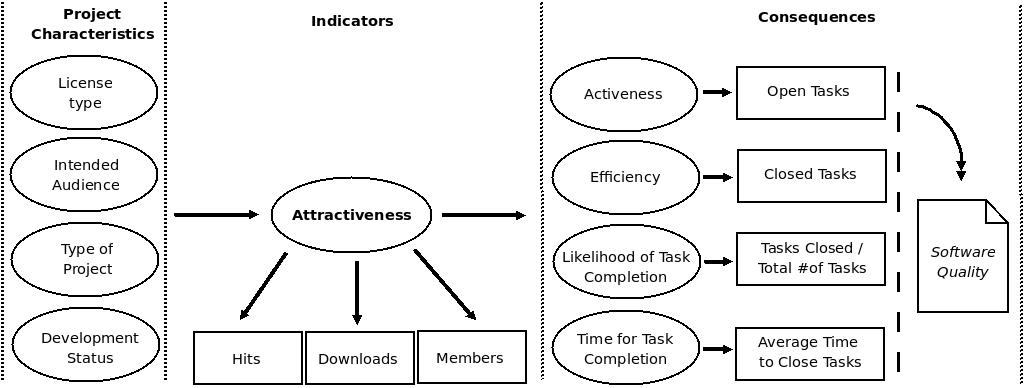
\includegraphics[scale=.45]{attractiveness}
\caption{Attractiveness research and measurement model}
\label{attractiveness}
\end{figure*}

Attractiveness is the capacity of bringing users and developers to a project.
%
A Free Software project is as much attractive as it has the ability to interest 
potential users and developers. They will later use the software and, ultimately, 
participate on tasks to improve the project \cite{Santos2010}.

In our study, the concept of attractiveness and its proxies are
based on Santos Jr.'s attractiveness model~\cite{Santos2010},
one of our previous works.
%
In this work is shown a research and measurement model for attractiveness,
presented in Figure~\ref{attractiveness}, that we started to expand and 
to adapted to our hypothesis about source code attributes and attractiveness.
%
This model defined project characteristics that influence 
its attractiveness, attractiveness indicators, 
and consequences of attractiveness (e.g., levels of activity, efficiency, 
likelihood of task completion, time for task completion, 
and software quality)~\cite{Santos2010}.


Originally, the project characteristics -- its typical origins -- proposed were:
\begin{itemize}
%
\item \emph{License Type} that a software was available such as GPL, BSD, 
and Mozilla Public.
%
The license influences the use and distribution of project and its rules for 
modifications because it regulates what can and cannot be done with the
source code and generated product~\cite{Santos2010}.

%
\item \emph{Intended audience} that is the kind of users (e.g., beginner, advanced)
and members (e.g., system administrator, Java programmers) of project.
%
Audience can influence the number of potential developers~\cite{johnson2002}.
%
However, audiences type can attract specific members, which define its expertise
and likelihood to contribute~\cite{Santos2010}.

%
\item \emph{Project type} refers a specific area that a projects might be related 
such as genealogy, payroll, browsing, games, scientific, etc~\cite{Crowston2002}.
%
Users focus on projects they judge to be more related to their work
and needs~\cite{johnson2002}, thereby project type influences their activities.
%
\item \emph{Life-cycle stage} -- development status -- that the software 
versions is available, for example, unstable, testing, production, and mature.
%
This status can influence developer's decisions to join and contribute to a
project~\cite{Santos2010}, what can affect members' motivations to release a
new version~\cite{raja2006,Stewart2006}. 

\end{itemize}

Therefore, we are proposing to insert source code attributes as a project
characteristics in this theoretical cause and effect model of Free Software
attractiveness, showed in Figure~\ref{attractiveness}.
%
For this, in ours study, we defined a simple (intermediary) attractiveness model
to observe individually the influence of source code attributes on the Free
Software attractiveness, presented in Figure~\ref{attractiveness2}.
%
In summary, a new cause that can partially explain attractiveness. We did not
deal to consequences of attractiveness when we added source code attributes as
a cause.

\begin{figure}[!t]
\centering
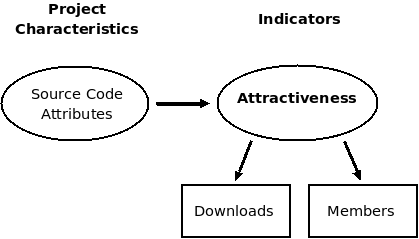
\includegraphics[scale=.45]{attractiveness2}
\caption{Attractiveness model: adapted proposal}
\label{attractiveness2}
\end{figure}


The attractiveness indicators can be estimated by the number of people that
joined the project and the number of software downloads.
%
This because before a Free Software project can receive failure reports, bug fixes, 
and new features, it should be attractive to volunteers, who normally first
join the project and later provide contributions.
%
Over time, these contributions affect the number of downloads and bring more 
members, creating a positive feedback loop.
%
Thus, we measured attractiveness based on the two empirical indicators:
\begin{enumerate}
\item \emph{number of downloads} is are presentation of the number of people
interested in the software.
\item \emph{number of members} represents the number of contributors to the project.
\end{enumerate}


One should note that the number of downloads and number of members
at SourceForge.net are simply proxies to the actual number of users and number of
developers in the project, respectively.
%
On the other hand, this study explored a large number of projects and applied 
the same criteria uniformly to all of them. 
%
Thereby, we did not find in previous works other proxies that can represent 
number of users and number of developers in a large sample of projects.

In conclusion, the meaning of ``successful'' to Free Software projects were
measured for different ways in previous rechearches:
%
(i) source code modularity (Shaikh and Cornford 2003);
(ii) number of lines of code generated (Mockus et al. 2000);
(iii) velocity of closing bugs (Stewart and Gosain 2006);
(iV) ability of a project to advance through development phases
(e.g., from alpha to beta to stable)~\cite{raja2006,Crowston2002};
(V) the number of downloads (Balijepally et al. 2009);
(vi) number of members (Crowston and Howison (2006).

Nos entendemos que essas medidas individualmente nao representem sucesso de forma completa, mas sim uma das formas de ajudar a chegar ao sucesso (ou mante-lo) quando analizadas juntas. Entretanto, no contexto do software livre, com o codigo-fonte sendo considerado o principal artefatos do projeto, levantamos a hipotese de que os atributos do codigo-fonte podem influenciar na atratividade do projeto, pois determinadas caracteristicas do codigo-fonte podem levar a mais contribuicoes ao software, atraindo mais usuarios e membros.


%-------------------------------------------------------------
\section{Research Design} 
\label{researchDesign}

Initially, this Section presents a source code analysis tool under development by our 
group called \texttt{Analizo} (Section~\ref{analizo}). It was used 
to calculate source code metric of 6,773 Free Software projects from SourceForge.net. 
%
Later, Section~\ref{sdcollection} presents the criteria used for sample and data collection. 
%
Finally, Section~\ref{variables} shows the multiple regression model defined 
to test our hypothesis, which are discussed in Section~\ref{hypotheses}.

\subsection{The Analizo Tool}
\label{analizo}

\texttt{Analizo}\footnote{\url{softwarelivre.org/mezuro/analizo}} is a 
multi-language source code analysis tool.
%
Its architecture was designed to support source code parsing, for different
languages, and to report useful information about it.

A basic requirement of our source code analysis tool was the ability to analyze
source code written in multiple languages.
%
Most existing tools use object code to extract data, making it impossible to process
projects that do not compile due to failures in either the source code or
in its dependencies~\cite{hassan05}.
%
In addition, tools based on object code are not
capable of analyzing features present only in the source, such as comments.
%
To avoid these problems, \texttt{Analizo} is designed to extract the information
directly from source code parsers.

\texttt{Analizo} uses \texttt{Doxyparse}\footnote{\url{softwarelivre.org/mezuro/doxyparse}},
a multi-language source code parser based on Doxygen's internals, to parse the source code.
%
This feature provides \texttt{Analizo} with the potential ability to parse all 
the languages supported by Doxygen\footnote{\url{doxygen.org}}, but, 
up to the moment, it has been tested only with C, C++, and Java source code.

\texttt{Analizo} has been fully tested with C source code downloaded from 
Sourceforge.net projects, supporting the computation of  fourteen metrics:
\begin{itemize}
\item \emph{Afferent Connections per Class} (ACC),
\item \emph{Coupling between Objects} (CBO),
\item \emph{Coupling Factor} (COF),
\item \emph{Depth of Inheritance Tree} (DIT),
\item \emph{Lack of Cohesion on Methods/Functions} (LCOM4),
\item \emph{Lines of Code} (LOC),
\item \emph{Lines per Method/Function} (AMZ\_Size),
\item \emph{Number of Attributes/Variables} (NOV),
\item \emph{Number of Children per Class} (NOC),
\item \emph{Number of Methods/Functions} (NOF),
\item \emph{Number of Classes/Module} (NM),
\item \emph{Number of Public Attributes/Variables} (NPV),
\item \emph{Number of Public Methods/Functions} (NPF),
\item \emph{Response for Class} (RFC).
\end{itemize}
The correctness of the metrics computation was evaluated by comparing the 
results provided by Analyzo and other existing tools such as
%
CCCC\footnote{\url{cccc.sourceforge.net}},
Cscope\footnote{\url{cscope.sourceforge.net}},
Eclipse-Metrics\footnote{\url{metrics.sourceforge.net}},
and Macxim/Spago4Q\footnote{\url{qualipso.dscpi.uninsubria.it/macxim}}.

%--------------------------------
\subsection{Sample and Data Collection}
\label{sdcollection}

%\vspace{-1em}
\begin{center}
\begin{table*}[hbt]
\centering \caption{Descriptive statistics}
\begin{tabular}{|l|r|r|r|r|r|r|} \hline
  & \multicolumn{4}{|c|}{Raw} & \multicolumn{2}{|c|}{Logarithm}\\ \hline

\textbf{Metric} & Min. & Max. & Mean & Std. Deviation & Mean & Std. Deviation \\ \hline

CBO & 0 & 7.12 & 2.26 & 9.04 & 0.35 & 0.98 \\ \hline

LCOM4 & 0 & 2.62 & 4.77 & 1.20 & 1.01 & 1.09 \\ \hline

SC & 0 & 4,940 & 15.79 & 114.69 & 1.37 & 1.57 \\ \hline

LOC & 11 & 2,983,103 & 17,700.00 & 91,614.70 & 8.28 & 1.58 \\ \hline

NM & 1 & 7,177 & 74.98 & 276.54 & 3.08 & 1.39 \\ \hline

Mbrs & 1 & 288 & 2.90 & 6.19 & 0.59 & 0.79 \\ \hline

Dls & 6 & 9,000,000 & 957,000.00 & 17,760,000.00 & 8.20 & 2.66 \\ \hline

\end{tabular}
\label{table:statistics}
\end{table*}
\end{center}
%\vspace{-1em}


SourceForge.net shares its data to support Free Software researchers.
%
In this study, we used the data available in a database managed by
the University of Notre Dame\footnote{\url{nd.edu/~oss/Data/data.html}}
and another one provided by the FLOSSMole project\footnote{\url{flossmole.org}}.
%
We accessed these databases in November, 2009 and collected data about
all the projects that matched the following criteria:
%
\begin{itemize}
\item \emph{Source code written in the C language}. 
While the vast majority of free software applications is written in
C \cite{robles2006:mining-large}, a large amount of research work
focuses their analyzes in projects written in Java (e.g. the related
work reported in section~\ref{related}).
%
Given this disparity between the actual free software ecosystem and
the research that address it, and our previous experience with
analysis of free software written in C \cite{terceiro2009}, we
choose to limit the analysis in this work to such projects as well.
%
This is our first study relating source code metrics and
attractiveness, and in the future we plan to include other
programming languages (e.g. C++, Java), as well as trying to
identify similarities and discrepancies among projects written in
different languages.
%%Chris: Daqueles 6% mencionados na secao 1, quantos projetos sao escritos em C?

\item \emph{More than one download}.  Projects with no downloads are
probably either non-development projects, or projects that have just started,
or are other special cases.
\end{itemize}

This provided us with a list of 11,433 projects. After this preliminary sampling,
the following steps were automatically executed  by scripts developed by our group,
to perform data collection:

\begin{enumerate}
\item Download the code of all the projects. This resulted in the source code 
for 10,128 projects since some of them had no available files (empty``files''
section in the SourceForge.net project pages);

\item Run \texttt{Analizo} sequentially for all projects and store the computed metrics in a single database.
%

The metrics were successfully computed for 6,773 projects only, because
(i) some downloaded files did not contain source code (e.g., binary-only downloads),
%
(ii) the source code was not written in C, (the project was incorrectly 
classified as being written in C), or
%
(iii) some files could not be processed by \texttt{Analizo} due to severe
errors in the source code (e.g., infinite loops);

\item Cross-joined the two datasets. Finally the two datasets --
the SourceForge.net data available from the University of Notre Dame and 
FLOSSMole on the one side and the source code metrics calculated 
by \texttt{Analizo} on the other side --  were cross-joined so that
we could perform the needed statistical analysis. 
\end{enumerate}

Table \ref{table:statistics} summarizes our sample, but the complete data set
used for this study is available on the Web~\footnote{\url{ccsl.ime.usp.br/mangue/data}}.
%
Section~\ref{variables} discusses in details how we selected the variables
presented in Table~\ref{table:statistics}.
%
This table shows natural values of minimum, maximum, arithmetic mean, and 
standard deviation for each variable, indicating the characteristics of our sample.

We analyzed our selected variables in their natural form (Raw) to verify their
distribution, which is presented in the first part of Table~\ref{table:statistics}.
%
Thereby, we observe that the Skewness and Kurtosis probability distribution
showed high values, indicating non-normality~\cite{hair2006}.
%
Because of this non-normality, we transformed the variables to a logarithm 
scale for linearization, which reduced the Skewness and Kurtosis values and made
them proper to run multiple regressions~\cite{Crowston2002}.
%
The arithmetic mean and standard deviation of the logarithm values can be
seen in the second part of Table~\ref{table:statistics}.
%% Paulo: writing center: in the ou in first/second part of ..

%--------------------------------
\subsection{Variables}
\label{variables}

Among the fourteen source code metrics that~\texttt{Analizo} provided, 
we selected seven for our initial analysis: 
%
total LOC, total NM,average NOF, average NPV, average NPF, average LCOM4,
and average CBO.
%
Since it is possible to generalize the concepts of ``class'' and ``method''
to ``module'' and ``function'', respectively, NOF, NPV, NPF, LCOM4 and CBO 
were applied to the procedural paradigm of the C language. 
%%\TODO Chris pediu referencia AQUI, mas nao vou ter tempo. 
%%Talvez o Terceiro tenha. Antes a ideia disso estava numa nota de rodape

In cases of ACC, AMZ\_Size, COF, DIT, NOC, NOV, and RFC metrics are not used 
because the source code attributes that they measure are not in the scope of this study.
%
We needed to limit the scope to accomplish the study. Thereby, we selected an initial 
subset of source code metrics based in the criteria that we wanted a simple
statistical model with size and complexity structural metrics. 
%
Therefore, in this first study, we disregard some other metrics.

%\vspace{-3em}
\begin{center}
\begin{table*}[hbt]
\centering \caption{Parametric Correlations: Pearson}
\begin{tabular}{|l|c|c|c|c|c|c|c|c|c|c|} \hline

\textbf{Variable} & CBO & LCOM4 & SC & NM & LOC & NPA & NOM & NPM & Mbrs & DLs
\\ \hline
CBO & - & 0.141 & 0.723 & 0.380 & 0.608 & 0.423 & 0.434 & 0.492 & 0.113 & 0.129
\\ \hline
LCOM4 & 0.141 & - & 0.786 & 0.019 & 0.472 & 0.102 & 0.311 & 0.361 & 0.080 & 0.107
\\ \hline
SC & 0.723 & 0.786 & - & 0.254 & 0.666 & 0.338 & 0.493 & 0.564 & 0.127 & 0.156
\\ \hline
NM & 0.308 & 0.019 & 0.254 & - & 0.799 & 0.730 & 0.815 & 0.827 & 0.311 & 0.344
\\ \hline
LOC & 0.608 & 0.472 & 0.666 & 0.799 & - & \textbf{0.872} & \textbf{0.923} & \textbf{0.927} & 0.328 & 0.410
\\ \hline
NPA & 0.423 & 0.102 & 0.338 & 0.730 & \textbf{0.872} & - & 0.756 & 0.761 & 0.303 & 0.386
\\ \hline
NOM & 0.434 & 0.311 & 0.493 & 0.815 & \textbf{0.923} & 0.756 & - & 0.886 & 0.320 & 0.380
\\ \hline
NPM & 0.492 & 0.361 & 0.564 & 0.827 & \textbf{0.927} & 0.761 & 0.886 & - & 0.308 & 0.365
\\ \hline
Mbrs & 0.113 & 0.080 & 0.127 & 0.311 & 0.328 & 0.303 & 0.320 & 0.308 & - & 0.676
\\ \hline
DLs & 0.129 & 0.107 & 0.156 & 0.344 & 0.410 & 0.386 & 0.380 & 0.365 & 0.676 & -
\\ \hline
\end{tabular}
\label{pearson}
\scalefont{1}
\end{table*}
\end{center}

%\vspace{-1em}
\begin{center}
\begin{table*}[bt]
\centering \caption{Non-Parametric Correlations: Spearman}
\begin{tabular}{|l|c|c|c|c|c|c|c|c|c|c|} \hline

\textbf{Variable} & CBO & LCOM4 & SC & NM & LOC & NPA & NOM & NPM & Mbrs & DLs
\\ \hline
CBO & - & 0.340 & 0.803 & 0.473 & 0.662 & 0.523 & 0.518 & 0.566 & 0.156 & 0.169
\\ \hline
LCOM4 & 0.340 & - & 0.773 & 0.213 & 0.490 & 0.348 & 0.478 & 0.516 & 0.129 & 0.162
\\ \hline
SC & 0.803 & 0.773 & - & 0.370 & 0.685 & 0.478 & 0.571 & 0.631 & 0.164 & 0.196
\\ \hline
NM & 0.473 & 0.213 & 0.370 & - & 0.793 & 0.718 & 0.818 & 0.828 & 0.284 & 0.320
\\ \hline
LOC & 0.662 & 0.490 & 0.685 & 0.793 & - & \textbf{0.863} & \textbf{0.918} & \textbf{0.922} & 0.307 & 0.392
\\ \hline
NPA & 0.523 & 0.348 & 0.478 & 0.718 & \textbf{0.863} & - & 0.758 & 0.765 & 0.280 & 0.363
\\ \hline
NOM & 0.518 & 0.478 & 0.571 & 0.818 & \textbf{0.918} & 0.758 & - & 0.895 & 0.300 & 0.362
\\ \hline
NPM & 0.566 & 0.516 & 0.631 & 0.828 & \textbf{0.922} & 0.765 & 0.895 & - & 0.288 & 0.347
\\ \hline
Mbrs & 0.156 & 0.129 & 0.164 & 0.284 & 0.307 & 0.280 & 0.300 & 0.288 & - & 0.598
\\ \hline
DLs & 0.169 & 0.162 & 0.196 & 0.320 & 0.392 & 0.363 & 0.362 & 0.347 & 0.598 & -
\\ \hline
\end{tabular}
\label{spearman}
\end{table*}
\end{center}

%\vspace{-1em}
\begin{center}
\begin{table*}[bt]
\centering \caption{Non-Parametric Correlations: Kendall}
\begin{tabular}{|l|c|c|c|c|c|c|c|c|c|c|} \hline

\textbf{Variable} & CBO & LCOM4 & SC & NM & LOC & NPA & NOM & NPM & Mbrs & DLs
\\ \hline
CBO & - & 0.244 & 0.650 & 0.341 & 0.483 & 0.377 & 0.373 & 0.410 & 0.118 & 0.114
\\ \hline
LCOM4 & 0.244 & - & 0.597 & 0.148 & 0.341 & 0.240 & 0.333 & 0.362 & 0.097 & 0.109
\\ \hline
SC & 0.650 & 0.597 & - & 0.262 & 0.497 & 0.345 & 0.413 & 0.460 & 0.124 & 0.132
\\ \hline
NM & 0.341 & 0.148 & 0.262 & - & 0.605 & 0.546 & 0.641 & 0.648 & 0.217 & 0.219
\\ \hline
LOC & 0.483 & 0.341 & 0.497 & 0.605 & - & \textbf{0.660} & \textbf{0.763} & \textbf{0.771} & 0.233 & 0.270
\\ \hline
NPM & 0.377 & 0.240 & 0.345 & 0.546 & \textbf{0.660} & - & 0.588 & 0.596 & 0.213 & 0.249
\\ \hline
NOM & 0.373 & 0.333 & 0.413 & 0.641 & \textbf{0.763} & 0.588 & - & 0.864 & 0.228 & 0.248
\\ \hline
NPM & 0.410 & 0.362 & 0.460 & 0.648 & \textbf{0.771} & 0.596 & 0.864 & - & 0.219 & 0.237
\\ \hline
Mbrs & 0.118 & 0.097 & 0.124 & 0.217 & 0.233 & 0.213 & 0.228 & 0.219 & - & 0.471
\\ \hline
DLs & 0.114 & 0.109 & 0.132 & 0.219 & 0.270 & 0.249 & 0.248 & 0.237 & 0.471 & -
\\ \hline
\end{tabular}
\label{kendall}
\end{table*}
\end{center}
%\vspace{-4em}

Nevertheless, in the first stage of our statistical analysis, LOC, NOM, NPA and NPM metrics 
showed high correlation between each other, according to Pearson's
parametric correlations shown in the Table~\ref{pearson}.
%
Highly correlated variables indicate that they are representations (partly) of
a same attribute, thereby making it unnecessary to use more than one.
%
Since all these metrics represent a similar concept, we selected one of them -- LOC -- 
for our statistical analysis to reduce multicollinearity.

We have also analyzed the Spearman and Kendal non-parametric correlations,
Table~\ref{spearman} and Table~\ref{kendall} respectively, given that some of
our variables are not normally distributed. 
%
In our analysis, we observed that after transforming our variables in their logarithmic form, 
Pearson correlations performed just as well as the non-parametric indices.
%
Thus, we chose the Pearson parametric correlation because it represents the most 
commonly used form of correlation index, and it also provides the basis for the 
regression analysis we performed later. That way, we could maintain
consistency because multiple regression techniques are based on
parametric indices~\cite{hair2006}.

According to analysis described above, we ended up considering LOC and NM 
as size metrics. Theoretically, the more LOC, the more NM.
%
However, it is possible to have more lines of code without having more modules, by
adding code into existing modules. Also, a software could have more modules
but keep the number of lines of code when refactoring is applied.
%
Furthermore, we understood that \emph{number of modules} (NM) did not highly
correlate with the others, since we considered a high correlation when the
Pearson's correlations values were approximately 0.9 or higher as our criteria,
emphasized in Table~\ref{pearson}.

%
In conclusion, LOC and NM measure different kinds of size metrics, more or less
influenced by programming languages and coding styles, respectively.
%
Thereby, we collected both the LOC and NM metrics.

Finally, CBO and LCOM4 were multiplied to obtain the value of our structural
complexity metric (SC), explained in Section~\ref{background}.
%
These three metrics did not show high correlations with other metrics.
%
As expected, SC showed a positive correlation with both. However, it was not 
as high as the others were, because CBO and LCOM4 had a low correlation
with each other. This means that SC, statistically, represents different attributes
when compared to CBO and LCOM4, thus endorsing  the theory that CBO and LCOM4 together
offer different information. 

In summary, our multiple regression model ended up with the following variables:

\begin{itemize}
\item \textbf{Independent variables (source code metrics)}
%
\begin{itemize}
\item \emph{Structural Complexity (SC)}: The product of CBO and LCOM4 metrics
%
\item \emph{Lines of Code (LOC)}, the sum of lines of code in all modules of the
project;
%
\item \emph{Number of Modules (NM)}, the total number of all modules of the project.
\end{itemize}

\item \textbf{Dependent variables (attractiveness)}
\begin{itemize}
\item \emph{Number of Downloads}: a proxy for the number of users of the
project;
%
\item \emph{Number of Members}: a proxy for the number of developers in the
project.
\end{itemize}
\end{itemize}

The model developed in this study revolves around attractiveness,
aiming at the explanation of its causes.
%
We defined a multiple regression model that has attractiveness as its dependent
variable. 
It was measured through two indicators: number of downloads and number of members. 
Thus, we have two different regressions, one for each attractiveness indicator.
%
They are the variables explained by the source code attributes proposed in our hypotheses.
%
Consequently, SC, LOC and MN metrics, which represent the source code attributes,
are the independent variables -- the influencers of attractiveness.

%----------------------------------------------------------------------

\subsection{Research Hypotheses} 
\label{hypotheses}

In this first study about the relationships between source code metrics and
attractiveness, we investigated whether two attributes -- structural complexity
and size -- obtained via four source code metrics might influence the attractiveness
of Free Software projects.
%
Thereby, we can later observe whether these attributes influence people's 
perception of quality as consequence of attractiveness.
%
Therefore, according to the metrics chosen to represent structural
complexity and size, we formulated three hypotheses:

\begin{enumerate}
\item \emph{Free Software projects with higher structural complexity have
lower attractiveness.}
%
The higher the software complexity, the more difficult it is to understand
its source code for maintenance and evolution purposes.
%
This leads to an increase in the maintenance effort, and makes it more
difficult to attract new members and users for the project.
%
Over time, with less members and users, the project may lose its ability to
add new features and fix bugs and, consequently, its ability to evolve and meet
the user's changing requirements.

\item \emph{Free Software projects with more lines of code have
higher attractiveness.}
%
To some extent, lines of code reflect the amount of features of the project and
the amount of work that have been put into it.
%
Therefore, projects with more lines of code will usually attract more users
(since they have more features) and developers -- since they offer more 
opportunities for contribution.

\item \emph{Free Software projects with a higher number of modules have
higher attractiveness.}
%
The number of modules may indicate the project size and the possibility
of working in parallel in independent modules.
%
More modules may indicate a concern with good design, with better modularization,
which facilitates contributions.
%
This attracts more members, who can write more features and fix more bugs,
which would then attract more users.
\end{enumerate}

%------------------------

\section{Hypotheses Testing}   
\label{hypothesesTesting}

%\vspace{-1em}
\begin{center}
\begin{table*}[hbt]
%\scalefont{0.9}
\centering \caption{Equations and Pearson Correlations}
\begin{tabular}{|l|r|r|r|r|r|r|r|r|} \hline

& \multicolumn{4}{|c|}{Downloads} & \multicolumn{4}{|c|}{Members}\\ \hline
  
\textbf{Metric} & $\beta$ & Std. $\beta$ & T-value & P-value & $\beta$ & Std. $\beta$ & T-value & P-value
\\ \hline
(Constant) & 1.551 & - & 6.12 & \textless 0.001 & -0.668 & - & -8.47 & \textless 0.001
\\ \hline
SC (log) & -0.286 & -0,150 & -8.616 & \textless 0.001 & -0.033 & -0.058 & -3.238 & 0.001
\\ \hline
LOC (log) & 0.856 & 0.506 & 18.624 & \textless 0.001 & 0.126 & 0.249 & 8.846 & \textless 0.001
\\ \hline
NM (log) & 0.008 & 0.004 & 0.186 & 0.852 & 0.087 & 0.148 & 6.625 & \textless 0.001
\\ \hline
   \hline
$R$ & \multicolumn{4}{|c|}{0.425} & \multicolumn{4}{|c|}{0.348}\\ \hline
$R^2$ & \multicolumn{4}{|c|}{0.180} & \multicolumn{4}{|c|}{0.121}\\ \hline
\end{tabular}
\label{table:regression}
\end{table*}
\end{center}
%\vspace{-2em}

%%TODO: new
We specified a multiple regression model to explain the relationships 
between the selected source code metrics and attractiveness in Free Software projects.
%
Before running this model, we analyzed and applied statistical techniques 
on the descriptive statistical values of our dataset presented in
Table~\ref{table:statistics}, discussed in Section~\ref{sdcollection}.
%
We selected the variable of our regression model according to our criteria for
definition of scope this study and analysis of the Pearson parametric
correlations, and Spearman and Kendal non-parametric correlations,
Table~\ref{pearson}, Table~\ref{spearman}, and Table~\ref{kendall} respectively,
presented in detail in Section~\ref{variables}.
%%TODO: new
Finally, with the linearized values of SC, NN, and LOC (independent variables) 
and number of downloads and number of members (dependent variables), we tested 
our hypotheses according to our statistical multiple regression model compound
for this variables.

Table~\ref{table:regression} summarizes the regression results based on the
Pearson's correlation values.
%
These statistical results indicated a linear dependency between our
source code metrics and each attractiveness variable.
%
In this table, $\beta$ is a coefficient that indicates the
size of the influence of each metric on each attractiveness indicator.

As we can see in Table~\ref{table:regression}, lines of code is more strongly
correlated to downloads and members than structural complexity and number of modules,
according to the standardized beta (\emph{Std. $\beta$}). 
%
Standardized betas are calculated to perform comparisons between variables that
are measured using different scales (e.g., lines of code and structural complexity).
One cannot compare regular beta coefficients without first standardizing them.

Moreover, structural complexity has a negative correlation with attractiveness,
as expected. Noteworthy is that T-test and P (probability) values represent whether a source code
metric is a statistically significant predictor or influencer of attractiveness indicators.
%
For downloads, the number of modules is not significant because
its P-value is greater than 0.05. 
%
Finally, in the last line of Table \ref{table:regression}, R-squared values
indicate the percentage of attractiveness (users and developers) variance that
this set of source code metrics is capable of explaining. 
%
So, roughly speaking, a R-squared of 20 percent indicates that a set of
predictors can explain 20 percent of a dependent variable.
%
We obtained the following equations:

\begin{displaymath}
\begin{array}{lll}
downloads = & 1.551 - 0.286\times log(SC) \\
            & + 0.856\times log(LOC) + 0.008\times log(NM) \\
\\
members = & -0.668 - 0.033\times log(SC) \\
            & + 0.126\times log(LOC) + 0.087\times log(NM)
\end{array}
\end{displaymath}

Each equation has one $R$-value. The coefficient ($\beta$) of each variable is
the size of influence that one of the source code metrics (the independent variable)
has on the attractiveness -- the dependent variable.
%
So, one unit change in an independent
variable generates a beta-size influence on the dependent variable, on average.


The $R$-value represents the amount of the dependent variables that can be
explained by that set of independent variables.
%
In our analysis, the $R$-value indicated that source code metrics explain 18\%
($R^2 = 0.180$) of the number of downloads and 12\% ($R^2 = 0.121$) of the
number of members. 
%
In conclusion, these are significant values for the social context that an
adoption or volunteering of a free software projects are involved.

\subsection{Hypothesis 1}

The data analysis supports our first hypothesis 
--~\emph{Free Software projects with higher structural complexity 
have lower attractiveness}.
%
In fact, structural complexity has a negative influence on attractiveness.
%
When related to downloads, it presents a -0.286 $\beta$ coefficient
and $p < 0.001$.
%
This means that structural complexity has an statistically significant impact on user interest.


In the Free Software context, structural complexity may indicate the
difficulty to make improvements to the software, such as new features and bug
fixes.
%
So, most users may loose interest in the software because another
project may have a greater capacity to meet their evolving needs.
%
Therefore, a smaller number of users, generating less reports could lead to 
less bug fixes and new features, which in turn could lead to less users in the future.


When related to members, structural complexity presents a $\beta$ of
-0.033 with $p = 0.001$, indicating that developers avoid to join
projects with high structural complexity.
%
A more complex source code is more difficult to understand and, consequently, 
to change.
%
This may prevent new developers from joining the project. With fewer members,
the community around a project is less active.
%\TODO{usar with ou and quando citar beta e p?}

\subsection{Hypothesis 2}

The second hypothesis --~\emph{Free Software projects with more
lines of code have higher attractiveness}~-- is also supported by our data.
Lines of code has a positive influence on attractiveness.


For downloads, this metric has $\beta = 0.856$, with $p<0.001$.
%
In this context, lines of code can be an indication of the amount of
software features and amount of work that have been put into the project so far.
%
The more features available, the more users will become interested in the project.
%
This may make the software more famous and more useful, attracting new members and users.


In addition, lines of code in relation to number of members indicated that
developers are interested in larger projects. The $\beta$ coefficient of
this metric for members is 0.126 ($p<0.001)$.
%
Therefore, for both downloads and members, lines of code is the metric with
the highest influence because it is associated with software features and project size.

\subsection{Hypothesis 3}

% part 1 - discuss the statistics
The most interesting results were related to our third hypothesis
--~\emph{Free Software projects with a higher number of modules have
higher attractiveness}.
%
For downloads, the data does not support the hypothesis: the high
$p$-value ( $p= 0.852$) does not allow us to claim that the number of
modules has any influence on the number of downloads.
%
For members, on the other hand, the hypothesis is confirmed: the number of modules
influences the number of members with $\beta = 0.087$, and $p<0.001$, which is
statistically significant.

% part 2 - discuss why the results are different for users and developers
Both lines of code and number of modules are metrics that represent software
size. The fact that both influence number of members, but only lines of codes
influence the number of downloads makes us wonder whether they represent
different characteristics of software size.
%
In this context, lines of code probably is related to the amount of features in the project, 
which helps to attract both users and developers to the project.


Additionally, when lines of code is kept constant, different values in
number of modules represent different ways of organizing these features over
different modules.
%
A higher number of modules thus indicates a higher modularity, which in turn makes
it easier for developers to work on the project, requiring less
coordination effort. This because is easier to work on modular software.
%
For users, on the other hand, it is probably the case that it does not matter
whether the software is modular or not; they are only interested in the provided features.

%conclusion
Finally, collaborators in Free Software projects often start participating in
the project as users, attracted by the software features.
%
After that, those users who have the potential to become developers may begin
to contribute code.
%
While a high number of lines of code (and thus of features) is enough to attract
users, project leaders should pay attention to source code quality.
%
To turn users into developers, the project has to provide a source code that is
easy to understand and modify by keeping structural complexity as low as possible
and modularity at a good level.

%----------------------------------------------------------------------------
\section{Related Work}
\label{related}

Large Free Software projects such as Debian GNU/Linux, GNOME, and KDE have invested in the
creation of dedicated teams for quality assurance. These efforts involve everything
from removing bugs and obsolete components to the definition of standards
and strategies to prevent bugs and improve quality \cite{Michlmayr2005}.
However, most projects do not have the resources to have a dedicated quality
team.
%
Michlmayr \emph{et al.} \cite{Michlmayr2005} performed a study on quality
assurance problems in Free Software such as unsupported code, configuration management,
security updates, users not knowing how to report bugs, the difficulty in
attracting volunteers, lack of documentation, and problems with coordination
and communication. None of these problems, however, are related to the quality
of the source code \emph{per se}.

Barkmann \emph{et al.} \cite{Barkmann2009} analyzed 146 Free Software projects
written in Java, identifying the correlation between a set of object-oriented
metrics and their theoretical ideal values. 
%
However, in their work the values of source code metrics were not associated
with problems or attractiveness of Free Software projects.

Stamelos \emph{et al.} \cite{Stamelos2002} presented empirical results on the relationship
between the size of application components and the delivered quality
measured as user satisfaction.
%
Quality characteristics of 100 applications written for GNU/Linux were compared to
industrial standards. The results indicated that the so-called structural
quality (e.g., component size) of an application is related to user satisfaction.

Midha \cite{midha2008} analyzed 450 projects from SourceForge.net and
verified that high values of MacCabe's Cyclomatic Complexity and
Haltead's Effort (complexity metrics) are positively correlated
with the number of bugs and with the time needed to fix bugs.
%
These metrics were also found to be negatively correlated with
contributions from new developers, i.e., more complex code is less
likely to attract new developers. However, Midha's study used complexity metrics
measured at the subroutine level, while in our study we use
complexity metrics at the module level.

Capra \emph{et al.} \cite{capra2008} have shown that open governance is associated
with higher software design quality on a study with 75 Free Software projects.
They defined software design quality in terms of 5 Object-Oriented metrics,
of which only CBO is used in our study.
%
An open governance structure together with the lack of formal management and
strict deadlines enables developers to enhance software design to have a
high-quality product, since they do not suffer pressure to release the 
software \cite{capra2008}.
%
Moreover, a better software design fosters a more open governance by allowing
developers to work in independent modules without the need for
explicit coordination activities. However, Capra's study has not addressed the
issue of attractiveness.

Bargallo \emph{et al.} \cite{bargallo2008} analyzed 56 Free Software projects,
studying the relationship between software design quality and project success.
%
They defined success in terms of downloads, page views and development activity,
and design quality in terms of the object-oriented metrics CBO, DIT, MIF, and NOC.
%
They found that the most successful projects exhibited lower design
quality. They argue that perhaps in successful projects the main
developers tend to shift their attention to lateral activities, such as
replying to users in forums, instead of focusing on enhancing the code quality.
%
Our results seemed to contradict theirs, but this is not the case. First, their
conceptualization of success is different from our conceptualization of
attractiveness.
%
Moreover, we considered structural complexity in terms of CBO
and LCOM4 metrics together, while they used a different set of metrics to
represent the notion of design quality, having only CBO in common with
the present study. Therefore, a straightforward comparison between their study and ours is not so simple.

%-------------------------------------------------------------------------
\section{Conclusion}
\label{conclusion}

A systematic review of 63 empirical studies showed that there is little research
addressing the characteristics or properties of Free Software projects,
such as their quality, growth, and evolution \cite{Stol2009}.
%
Our study contributes with an unprecedented analysis of
source code metrics from thousands of Free Software projects,
causally linking software source code characteristics with attractiveness.
%
In doing so, we expect to raise awareness on an important topic so far
neglected. Free Software projects fail when they lack attractiveness.
Therefore, understanding what influences attractiveness provides
managerial knowledge to project leaders, pointing them to the right
direction on prioritizing their resources.

Our results indicated that source code size and structural complexity
explain a relevant percentage of the attractiveness of Free Software projects.
%
Attractiveness is based on human perceptions and influenced by people's
cognition, making it a complex issue, hard to understand and explain
completely.
%
Nevertheless, our study was able to explain 18\% of software
users and 12\% of project developers, through a set of four source code metrics.
%
These statistical results are significant for the social context that
Free Software projects adoption and volunteering are inserted.

In this study, we showed that lines of code (LOC)
has a significant effect on the number of project users.
%
Our results also indicated that structural complexity (SC) has a negative
influence on project attractiveness.
%
Therefore, a project will face greater difficulties to grow without observing
some source code attributes such as cohesion, coupling, and modularity,
which favors developer contributions such as new features and bug fixes.

In other words, our analysis indicated that software structural complexity growth
may decrease the positive effects of new added features on attractiveness.
%
Ideally, a project should keep its complexity constant as new code is incorporated,
because developers are interested in improving the software, and the users in the improvements.
%
This demonstrates to project leaders (in communities, foundations,
governments, and companies)
the importance to monitor LCOM4 and CBO metrics together with NM and LOC,
thereby increasing their chances of forming a community of contributors
around their software, further enhancing its quality.
Thus, projects should grow managing their complexity, keeping the new
members willingness to contribute.

Our study differs from related work because we analyzed a large
sample of Free Software projects. Table \ref {table:statistics} shows how diverse our sample of
6,773 projects is. There are projects with thousands of modules (7,177),
millions of lines of code (2,983,103), large structural complexity (4,940),
several hundred members (288), and millions of downloads (9,000,000).
This sample was based on well-defined criteria and the number of projects
involved provided us with statistical confidence in the results.

Nevertheless, this study has some limitations that motivate future work.
%
Our sample is restricted to projects written in C available at
SourceForge.net and our analysis to a limited set of metrics.
In the future, we will include projects from other repositories, and extend
this study to other source code metrics and programming languages such as C++
and Java. 
%
Furthermore, widely known projects such as GNU/Linux and Firefox should be
included in studies of this kind, for their metrics may signal references
needing to be followed.
%% Chris : references needing to be followed????
%% Paulo: nao ... estamos especulando ;)

Finally, we acknowledge that source code metrics are not the only
variables capable of influencing attractiveness.
%
Our previous work has identified that things such as the restrictiveness of
the license, type of project, software life-cycle stage, and intended audience
are all capable of influencing attractiveness \cite{Santos2010}.
%
At first sight, assuming that all these variables from our previous study are
independent from the source code metrics we studied here, roughly 40\% of attractiveness variance would be then explained.
%
However, including variables in an equation in a statistically sound manner is not
straightforward. Accordingly, there is a need to further identify the interaction
between that set of variables with the ones reported in this study.

\section*{Acknowledgments}
The authors of this paper are supported by CNPQ, FAPESP, and the Qualipso project.
This research has been developed in the USP Free Software Competence Center and the
authors would like to thank Claudia Melo, Lucianna Almeida, Joenio Costa,
Beraldo Leal, and Nelson Lago for their contributions.

\bibliographystyle{IEEEtran}
\bibliography{../myReferences}
\end{document}
